\documentclass[border=10pt]{standalone}
\usepackage{pgfplots}
\usepgfplotslibrary{fillbetween}
\pgfplotsset{compat=1.18}
\begin{document}
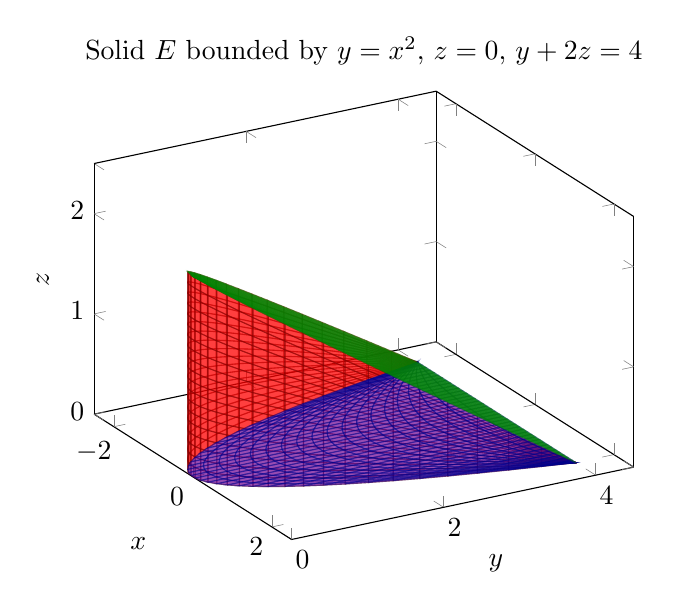
\begin{tikzpicture}
\begin{axis}[
    view={60}{30},
    xlabel=$x$, ylabel=$y$, zlabel=$z$,
    samples=40, samples y=20,
    xmin=-2.5, xmax=2.5,
    ymin=0, ymax=4.5,
    zmin=0, zmax=2.5,
    title={Solid $E$ bounded by $y=x^2$, $z=0$, $y+2z=4$},
]
\addplot3[surf, opacity=0.5, red, faceted color=red!50!black, domain=-2:2, y domain=0:1] (x, {x^2}, {y*(2-x^2/2)});
\addplot3[surf, opacity=0.4, blue, faceted color=blue!50!black, domain=-2:2, y domain=0:1] (x, {x^2 + y*(4-x^2)}, 0);
\addplot3[surf, opacity=0.4, green!60!black, faceted color=green!50!black, domain=0:2, y domain=-1:1] ({y*sqrt(4-2*x)}, {4-2*x}, {x});
\end{axis}
\end{tikzpicture}
\end{document}